\documentclass[11pt,a4paper]{article}

\usepackage[a4paper,margin=1in]{geometry}
\usepackage{fontspec}
\usepackage{xeCJK}
\usepackage{amsmath,amssymb,bm}
\usepackage{booktabs}
\usepackage{enumitem}
\usepackage{graphicx}
\usepackage{hyperref}

\setmainfont{Times New Roman}
\setCJKmainfont{SimSun}
\setCJKsansfont{Microsoft YaHei}
\setmonofont{Consolas}

\hypersetup{
    colorlinks=true,
    linkcolor=blue,
    urlcolor=blue,
    citecolor=blue
}

\title{一种从半线性端点到 Monge--Amp\`ere 方程的\\Legendre--Galerkin 同伦原型方法}
\author{Codex 实验说明稿}
\date{March 23, 2026}

\begin{document}
\maketitle

\begin{abstract}
本文整理一类从半线性端点到 Monge--Amp\`ere 方程的同伦 Legendre--Galerkin 原型方法，用于求解二维正方形区域上的 Dirichlet 问题
\[
\det(D^2u)=f.
\]
与 $u_0$ 锚定同伦不同，这里考虑新的连续同伦族
\[
t(\Delta u+u^3)+(1-t)\det(D^2u)=f,\qquad t\in[0,1],
\]
其中 $t=1$ 对应半线性端点 $\Delta u+u^3=f$，$t=0$ 对应目标 Monge--Amp\`ere 方程。为提高 $t=1$ 层求解的稳定性，代码先用 Poisson 型方程构造 warm start，再沿辅助参数 $s\in[0,1]$ 求解一族 bootstrap 方程
\[
\Delta u+s\,u^3=f.
\]
本文给出该方法的数学模型、边界 lifting、Legendre--Galerkin 离散、残差分解、解析 Jacobian、continuation 与凸性诊断策略，并整理 \texttt{quartic\_convex} 与 \texttt{paper\_example\_5\_1} 两组算例的数值结果。实验表明，在当前默认参数下，指数型光滑凸解算例可以稳定收敛到 $t=0$，而四次多项式凸解算例在半线性端点求解阶段即出现失稳，反映了该新同伦路径当前的适用边界。
\end{abstract}

\noindent\textbf{关键词：}
Monge--Amp\`ere 方程；半线性同伦；Legendre--Galerkin 方法；边界 lifting；bootstrap 初始化；解析 Jacobian

\section{引言}
Monge--Amp\`ere 方程
\begin{equation}
\det(D^2u)=f
\label{eq:ma}
\end{equation}
是典型的全非线性二阶偏微分方程。其数值求解不仅受到全非线性结构的影响，还与凸性分支选择、初值质量以及离散空间中非线性项的逼近方式密切相关。对于谱方法而言，空间逼近精度往往较高，但 Newton 迭代是否能够进入正确分支，仍然强烈依赖于连续层面的求解路径设计。

现有原型中，一种可行路径是采用 $u_0$ 锚定同伦，通过
\[
t(u-u_0)+(1-t)(\det(D^2u)-f)=0
\]
逐层从锚定态过渡到 Monge--Amp\`ere 端点。本文关注另一条同伦理路：不再直接锚定到某个参考解，而是将一个相对温和的半线性端点
\[
\Delta u+u^3=f
\]
作为起始问题，再经由参数 $t$ 连续过渡到 Monge--Amp\`ere 方程。这样做的动机在于：半线性端点仍保留了与目标方程一致的边界数据，但其 Jacobian 结构更易控制；另一方面，若半线性端点足够接近目标凸解分支，则 continuation 可能提供一条新的可计算通道。

与此对应，本文所整理的 MATLAB 原型文件保留了稳定的 Legendre--Galerkin 基函数、B-matrix 变换链、边界 lifting、解析 Hessian 行列式 Jacobian 与凸性诊断框架，但将连续模型替换为新的半线性同伦族，并引入一个 bootstrap 初始化阶段，以便更稳妥地抵达 $t=1$ 层。本文重点说明该原型的数学结构与数值表现，而不宣称尚未建立的严格收敛性理论。

\section{模型问题与初始化策略}
\subsection{半线性到 Monge--Amp\`ere 的同伦模型}
考虑正方形区域
\[
\Omega=(0,1)^2
\]
及 Dirichlet 边界条件
\begin{equation}
u=g \qquad \text{on }\partial\Omega.
\label{eq:bc}
\end{equation}
本文中的同伦模型为：对任意固定 $t\in[0,1]$，求解
\begin{equation}
t(\Delta u_t+u_t^3)+(1-t)\det(D^2u_t)=f
\qquad \text{in }\Omega,
\label{eq:homotopy}
\end{equation}
并配以边界条件
\begin{equation}
u_t=g \qquad \text{on }\partial\Omega.
\label{eq:bc-t}
\end{equation}
显然，当 $t=1$ 时，方程 \eqref{eq:homotopy} 退化为半线性端点问题
\begin{equation}
\Delta u+u^3=f;
\label{eq:semi-endpoint}
\end{equation}
当 $t=0$ 时，恢复目标方程 \eqref{eq:ma}。

实际计算中，取参数序列
\begin{equation}
1=t_0>t_1>\cdots>t_K=0,
\label{eq:t-sequence}
\end{equation}
并逐层进行 continuation。若在 $t=t_k$ 层获得可接受近似，则将其用作下一层 $t=t_{k+1}$ 的初值。代码中继续采用自适应步长缩放：若某一层收敛则增大步长，若失败则减半重试，直到到达 $t=0$ 或低于最小步长阈值。

\subsection{边界 lifting}
为了在谱空间中处理非齐次 Dirichlet 边界条件，将解写成
\begin{equation}
u_t=U_t+U_b,
\label{eq:split}
\end{equation}
其中 $U_b$ 为 lifting，满足
\[
U_b=g \qquad \text{on }\partial\Omega,
\]
而未知量 $U_t$ 满足齐次边界条件
\[
U_t=0 \qquad \text{on }\partial\Omega.
\]
与前一篇 $u_0$ 锚定论文相同，这里采用由四条边界数据拼接得到的双线性延拓
\begin{align}
U_b(x,y)
= {} & (1-x)g(0,y)+xg(1,y) \notag \\
& +(1-y)\bigl(g(x,0)-(1-x)g(0,0)-xg(1,0)\bigr) \notag \\
& +y\bigl(g(x,1)-(1-x)g(0,1)-xg(1,1)\bigr),
\label{eq:ub}
\end{align}
从而保证四条边界上一致满足给定边值。

记
\[
V:=H^2(\Omega)\cap H_0^1(\Omega),
\]
则在总场 $u_t=U_t+U_b$ 的表达下，连续投影形式可写为：求 $U_t\in V$，使得
\begin{equation}
t(\Delta u_t+u_t^3,v)+(1-t)(\det(D^2u_t),v)=(f,v),
\qquad \forall v\in V,
\label{eq:weak-cont}
\end{equation}
其中 $(\cdot,\cdot)$ 表示 $L^2(\Omega)$ 内积。这里并未对 Laplace 项作分部积分，而是保持强形式投影；这与后续代码中的矩阵组装方式保持一致。

\subsection{Poisson warm start 与 bootstrap 初始化}
虽然同伦端点 \eqref{eq:semi-endpoint} 比 Monge--Amp\`ere 方程更温和，但直接从任意初值求解它仍可能较困难。为此，代码首先构造 Poisson 型 warm start：
\begin{equation}
\Delta u_{\mathrm{init}} = 2\sqrt{f},
\qquad
u_{\mathrm{init}}=g \quad \text{on }\partial\Omega.
\label{eq:warmstart}
\end{equation}
该步骤仅用于给出一个较平滑的初始场，并不构成本方法的主要同伦端点。

在得到 $u_{\mathrm{init}}$ 后，代码并不立即求解 \eqref{eq:semi-endpoint}，而是沿辅助参数 $s\in[0,1]$ 求解一族 bootstrap 方程
\begin{equation}
\Delta u+\;s\,u^3=f,
\qquad
u=g \quad \text{on }\partial\Omega.
\label{eq:bootstrap}
\end{equation}
默认参数下，
\begin{equation}
s\in\{0,0.1,0.2,\dots,1.0\}.
\label{eq:s-seq}
\end{equation}
每一层 $s=s_j$ 的数值解被用作下一层 $s=s_{j+1}$ 的 Newton 初值；当 $s=1$ 成功求解后，其结果就作为主同伦 \eqref{eq:homotopy} 在 $t=1$ 层的初值。代码中这一阶段由 \texttt{solve\_semilinear\_bootstrap} 实现，对应的残差与 Jacobian 将在后文给出。

\section{Legendre--Galerkin 离散、残差与 Jacobian}
\subsection{参考区域映射与离散空间}
引入参考区域
\[
\widehat\Omega=(-1,1)^2
\]
及线性映射
\begin{equation}
x=\frac{\xi+1}{2},
\qquad
y=\frac{\eta+1}{2}.
\label{eq:map}
\end{equation}
由链式法则可得
\begin{equation}
\partial_{xx}=4\partial_{\xi\xi},
\qquad
\partial_{yy}=4\partial_{\eta\eta},
\qquad
\partial_{xy}=4\partial_{\xi\eta},
\label{eq:scaling}
\end{equation}
以及
\begin{equation}
\det(D^2_{x,y}u)=16\,\det(D^2_{\xi,\eta}u).
\label{eq:det-scale}
\end{equation}
因此方程 \eqref{eq:homotopy} 在参考区域上化为
\begin{equation}
t\Bigl[\frac14\bigl(u_{\xi\xi}+u_{\eta\eta}\bigr)+\frac1{16}u^3\Bigr]
+(1-t)\det(D^2_{\xi,\eta}u)
=\frac1{16}f.
\label{eq:ref}
\end{equation}

在区间 $(-1,1)$ 上取满足齐次边界条件的基函数
\begin{equation}
\phi_n(\xi)=L_n(\xi)-L_{n+2}(\xi),
\qquad n=0,1,\dots,N-1,
\label{eq:phi}
\end{equation}
其中 $L_n$ 为 Legendre 多项式。二维离散空间取为
\begin{equation}
X_N=\mathrm{span}\{\phi_i(\xi)\phi_j(\eta)\}_{i,j=0}^{N-1}.
\label{eq:space}
\end{equation}
若记
\begin{equation}
U_N(\xi,\eta)=\sum_{i,j=0}^{N-1}U_{ij}\phi_i(\xi)\phi_j(\eta),
\qquad
u_N=U_N+U_b,
\label{eq:UN}
\end{equation}
则数值未知量为系数向量
\[
\bm U=\mathrm{vec}\bigl([U_{ij}]_{i,j=0}^{N-1}\bigr)\in \mathbb{R}^{N^2}.
\]

再记 $\{(\xi_p,\omega_p)\}_{p=1}^Q$ 为一维 Legendre--Gauss 节点与权重，并定义二维离散内积
\begin{equation}
(w,z)_Q=\sum_{p=1}^Q\sum_{q=1}^Q w(\xi_p,\eta_q)z(\xi_p,\eta_q)\omega_p\omega_q.
\label{eq:quad}
\end{equation}
则主同伦问题的离散形式为：对任意固定 $t\in[0,1]$，求 $U_N(t)\in X_N$，使得
\begin{equation}
t\Bigl[\frac14(u_{\xi\xi}+u_{\eta\eta},v_N)_Q+\frac1{16}(u_N^3,v_N)_Q\Bigr]
+(1-t)(\det(D^2_{\xi,\eta}u_N),v_N)_Q
=\frac1{16}(f,v_N)_Q
\label{eq:weak}
\end{equation}
对一切 $v_N\in X_N$ 成立。

\subsection{B-matrix 变换链}
代码与旧原型相同，仍采用 B-matrix 变换链组织离散算子。设
\[
\Phi_q=[\phi_j(\xi_p)]_{p,j},
\qquad
T_0=\Phi_q\otimes \Phi_q,
\]
则 $T_0$ 将谱系数映射到 quadrature 节点值。另一方面，一维离散投影矩阵记为
\[
P_\phi=B_3^\top B_2B_1,
\]
对应的二维投影算子为
\begin{equation}
T_1=P_\phi\otimes P_\phi.
\label{eq:T1}
\end{equation}
此外，借助 Legendre 多项式导数递推构造二阶导数算子
\begin{equation}
T_2=(P_q\otimes P_q)(I\otimes B_5)(B_3\otimes B_3),
\label{eq:T2}
\end{equation}
\begin{equation}
T_3=(P_q\otimes P_q)(B_5\otimes I)(B_3\otimes B_3),
\label{eq:T3}
\end{equation}
\begin{equation}
T_4=(P_q\otimes P_q)(B_6\otimes B_6)(B_3\otimes B_3).
\label{eq:T4}
\end{equation}
若 lifting 的二阶导数节点值分别记为 $\bm u^{(b)}_{\xi\xi}$、$\bm u^{(b)}_{\eta\eta}$ 和 $\bm u^{(b)}_{\xi\eta}$，则总场在节点上的 Hessian 分量为
\begin{equation}
\bm u_{\xi\xi}=T_2\bm U+\bm u^{(b)}_{\xi\xi},
\qquad
\bm u_{\eta\eta}=T_3\bm U+\bm u^{(b)}_{\eta\eta},
\qquad
\bm u_{\xi\eta}=T_4\bm U+\bm u^{(b)}_{\xi\eta}.
\label{eq:hessian}
\end{equation}
此外，Poisson warm start \eqref{eq:warmstart} 的齐次部分离散为
\begin{equation}
L\bm U_{\mathrm{init}}=T_1\bm s,
\qquad
L=T_1(T_2+T_3),
\label{eq:poisson-discrete}
\end{equation}
这正对应代码中的 \texttt{ops.L}。

\subsection{残差分解}
为了与代码中的 \texttt{residual\_components} 一致，先定义节点值向量
\[
\bm u=T_0\bm U+\bm U_b^{(q)}.
\]
则 Laplace 项、立方项与 Hessian 行列式项在投影后的代数量分别为
\begin{equation}
\bm \ell=T_1(\bm u_{\xi\xi}+\bm u_{\eta\eta}),
\qquad
\bm c=T_1(\bm u^{\odot 3}),
\qquad
\bm d=T_1(\bm u_{\xi\xi}\odot \bm u_{\eta\eta}-\bm u_{\xi\eta}^{\odot 2}),
\label{eq:components}
\end{equation}
其中 $\odot$ 表示逐点乘积。右端投影记为
\begin{equation}
\bm F=T_1\bm f_q,
\qquad
\bm f_q=\frac1{16}[f(\xi_p,\eta_q)]_{p,q}.
\label{eq:F}
\end{equation}

于是半线性端点残差为
\begin{equation}
\bm A(\bm U)=\frac14\bm\ell+\frac1{16}\bm c-\bm F,
\label{eq:aux-res}
\end{equation}
Monge--Amp\`ere 端点残差为
\begin{equation}
\bm M(\bm U)=\bm d-\bm F,
\label{eq:ma-res}
\end{equation}
主同伦残差则写成
\begin{equation}
R_t(\bm U)=t\,\bm A(\bm U)+(1-t)\,\bm M(\bm U).
\label{eq:residual}
\end{equation}
这正对应 MATLAB 中
\[
\texttt{r = t\_val * aux\_vec + (1 - t\_val) * ma\_vec.}
\]

对于 bootstrap 阶段 \eqref{eq:bootstrap}，代码使用的阶段残差为
\begin{equation}
R^{(s)}_{\mathrm{boot}}(\bm U)=\frac14\bm\ell+\frac{s}{16}\bm c-\bm F.
\label{eq:boot-res}
\end{equation}
当 $s=1$ 时，它与半线性端点残差 \eqref{eq:aux-res} 完全一致。

\subsection{解析 Jacobian}
半线性端点残差 \eqref{eq:aux-res} 的 Jacobian 为
\begin{equation}
J_{\mathrm{aux}}(\bm U)
=
\frac14L+\frac1{16}T_1\mathrm{diag}(3\bm u^{\odot 2})T_0.
\label{eq:Jaux}
\end{equation}
bootstrap 阶段对应的 Jacobian 则为
\begin{equation}
J^{(s)}_{\mathrm{boot}}(\bm U)
=
\frac14L+\frac{s}{16}T_1\mathrm{diag}(3\bm u^{\odot 2})T_0.
\label{eq:Jboot}
\end{equation}

对于 Monge--Amp\`ere 项，利用 \eqref{eq:hessian} 可得
\[
\delta \bm u_{\xi\xi}=T_2\delta\bm U,\qquad
\delta \bm u_{\eta\eta}=T_3\delta\bm U,\qquad
\delta \bm u_{\xi\eta}=T_4\delta\bm U,
\]
从而
\begin{equation}
\delta \bm d
=
T_1\Bigl(
\mathrm{diag}(\bm u_{\eta\eta})T_2
+\mathrm{diag}(\bm u_{\xi\xi})T_3
-2\,\mathrm{diag}(\bm u_{\xi\eta})T_4
\Bigr)\delta\bm U.
\label{eq:det-var}
\end{equation}
因此其 Jacobian 为
\begin{equation}
J_{\det}(\bm U)
=
T_1\Bigl(
\mathrm{diag}(\bm u_{\eta\eta})T_2
+\mathrm{diag}(\bm u_{\xi\xi})T_3
-2\,\mathrm{diag}(\bm u_{\xi\eta})T_4
\Bigr).
\label{eq:Jdet}
\end{equation}
最终，主同伦残差 \eqref{eq:residual} 的 Jacobian 写成
\begin{equation}
J_t(\bm U)=t\,J_{\mathrm{aux}}(\bm U)+(1-t)\,J_{\det}(\bm U).
\label{eq:Jt}
\end{equation}
在实现层面，这一解析 Jacobian 由 \texttt{auxiliary\_jacobian} 与 \texttt{jacobian} 直接组装，而不是通过差分近似得到。

\section{Continuation、线搜索与分支诊断}
对每一层 $t=t_k$，Newton 校正量 $\delta\bm U$ 由
\begin{equation}
J_{t_k}(\bm U^{(m)})\delta\bm U=-R_{t_k}(\bm U^{(m)})
\label{eq:newton}
\end{equation}
给出。代码在每一步 Newton 迭代中都使用带回溯的线搜索，并额外引入凸性相关的接受准则。具体而言，除总残差下降外，还同时监控：
\begin{itemize}[leftmargin=2em]
\item Hessian 最小和最大特征值；
\item Hessian 半正定比例 $\mathrm{PSD\ ratio}$；
\item Hessian 不定比例 $\mathrm{indef\ ratio}$；
\item 行列式非负比例 $\mathrm{det\texttt{+}\ ratio}$。
\end{itemize}
只有当试探步在这些指标上不过度恶化，或总体评分有所改善时，该步才会被接受。该策略并不等价于严格的理论凸性约束，但在数值上有助于避免迭代偏离目标凸解分支。

\section{数值实验}
\subsection{实验设置}
本文使用代码默认参数：谱截断阶数 $N=32$，Legendre--Gauss 节点数 $Q=32$，评估网格点数为 $121\times121$，Newton 容差为 $10^{-10}$，层间接受阈值为 $10^{-8}$，最小 continuation 步长为 $2.5\times 10^{-3}$。bootstrap 阶段采用序列 \eqref{eq:s-seq}。

测试的两组 manufactured solution 与代码一致：
\begin{enumerate}[leftmargin=2em]
\item \texttt{quartic\_convex}
\[
u_{\mathrm{exact}}(x,y)=\frac{x^2+y^2}{2}+x^4+y^4,
\qquad
f=(1+12x^2)(1+12y^2);
\]
\item \texttt{paper\_example\_5\_1}
\[
u_{\mathrm{exact}}(x,y)=\exp\!\left(\frac{x^2+y^2}{2}\right),
\qquad
f=(1+x^2+y^2)\exp(x^2+y^2).
\]
\end{enumerate}

\begin{table}[htbp]
\centering
\caption{两组算例在默认参数下的最终结果概览}
\resizebox{\textwidth}{!}{%
\begin{tabular}{lccccccc}
\toprule
算例 & 成功 & 终止 $t$ & 总残差 & MA 残差 & Grid $L^2$ & PSD 比例 & det$+$ 比例 \\
\midrule
quartic\_convex & false & $1$ & $1.367\times 10^0$ & $1.124\times 10^1$ & $2.991\times 10^{-1}$ & $0.369$ & $0.369$ \\
paper\_example\_5\_1 & true & $0$ & $7.817\times 10^{-12}$ & $7.817\times 10^{-12}$ & $6.898\times 10^{-13}$ & $1.000$ & $1.000$ \\
\bottomrule
\end{tabular}
}
\label{tab:summary}
\end{table}

表 \ref{tab:summary} 显示，新同伦方法在两组算例上的表现差异明显。在指数型光滑凸解算例中，bootstrap 与主 continuation 都能稳定推进至 $t=0$；而在四次多项式凸解算例中，算法在最初的 bootstrap 阶段便未能通过默认的牛顿--线搜索--凸性筛选组合。

\subsection{\texorpdfstring{$paper\_example\_5\_1$}{paper example 5.1}: 成功收敛的算例}
对于 \texttt{paper\_example\_5\_1}，bootstrap 阶段从 $s=0$ 到 $s=1$ 全部收敛，总 Newton 步数为 $153$。随后主同伦从 $t=1$ 推进到 $t=0$，最终得到
\[
\|R_0\|_\infty = 7.817\times 10^{-12},
\qquad
\|M(\bm U)\|_\infty = 7.817\times 10^{-12},
\]
并且误差指标达到
\[
\text{Grid }L^2 = 6.898\times 10^{-13},\quad
\text{FD-}H^1 = 3.472\times 10^{-12},\quad
\text{FD-}H^2 = 1.628\times 10^{-10}.
\]
最终 Hessian 最小特征值约为 $2.500\times 10^{-1}$，PSD 比例与 det-positive 比例均为 $1$，说明数值解在整个 quadrature 网格上保持了良好的凸性结构。

\begin{table}[htbp]
\centering
\caption{\texttt{paper\_example\_5\_1} 的若干接受层结果}
\begin{tabular}{ccccc}
\toprule
$t$ & 总残差 & MA 残差 & Grid $L^2$ & PSD 比例 \\
\midrule
$1$ & $5.485\times 10^{-14}$ & $1.286\times 10^0$ & $1.984\times 10^{-1}$ & $0.000$ \\
$10^{-1}$ & $2.519\times 10^{-11}$ & $8.307\times 10^{-2}$ & $7.777\times 10^{-3}$ & $1.000$ \\
$10^{-3}$ & $1.567\times 10^{-11}$ & $7.822\times 10^{-4}$ & $7.200\times 10^{-5}$ & $1.000$ \\
$10^{-5}$ & $7.278\times 10^{-15}$ & $7.817\times 10^{-6}$ & $7.194\times 10^{-7}$ & $1.000$ \\
$0$ & $7.817\times 10^{-12}$ & $7.817\times 10^{-12}$ & $6.898\times 10^{-13}$ & $1.000$ \\
\bottomrule
\end{tabular}
\label{tab:paper-example}
\end{table}

表 \ref{tab:paper-example} 表明，该算例在从 $t=1$ 到 $t=0$ 的过程中迅速进入正确的凸解分支。特别地，虽然 $t=1$ 层的半线性端点解本身并不是目标 Monge--Amp\`ere 解，故其 MA 残差约为 $1.286$，但只要 $t$ 下降到 $10^{-1}$，PSD 比例便恢复到 $1$，而误差和 MA 残差都以近似线性的数量级迅速下降。

\begin{figure}[htbp]
\centering
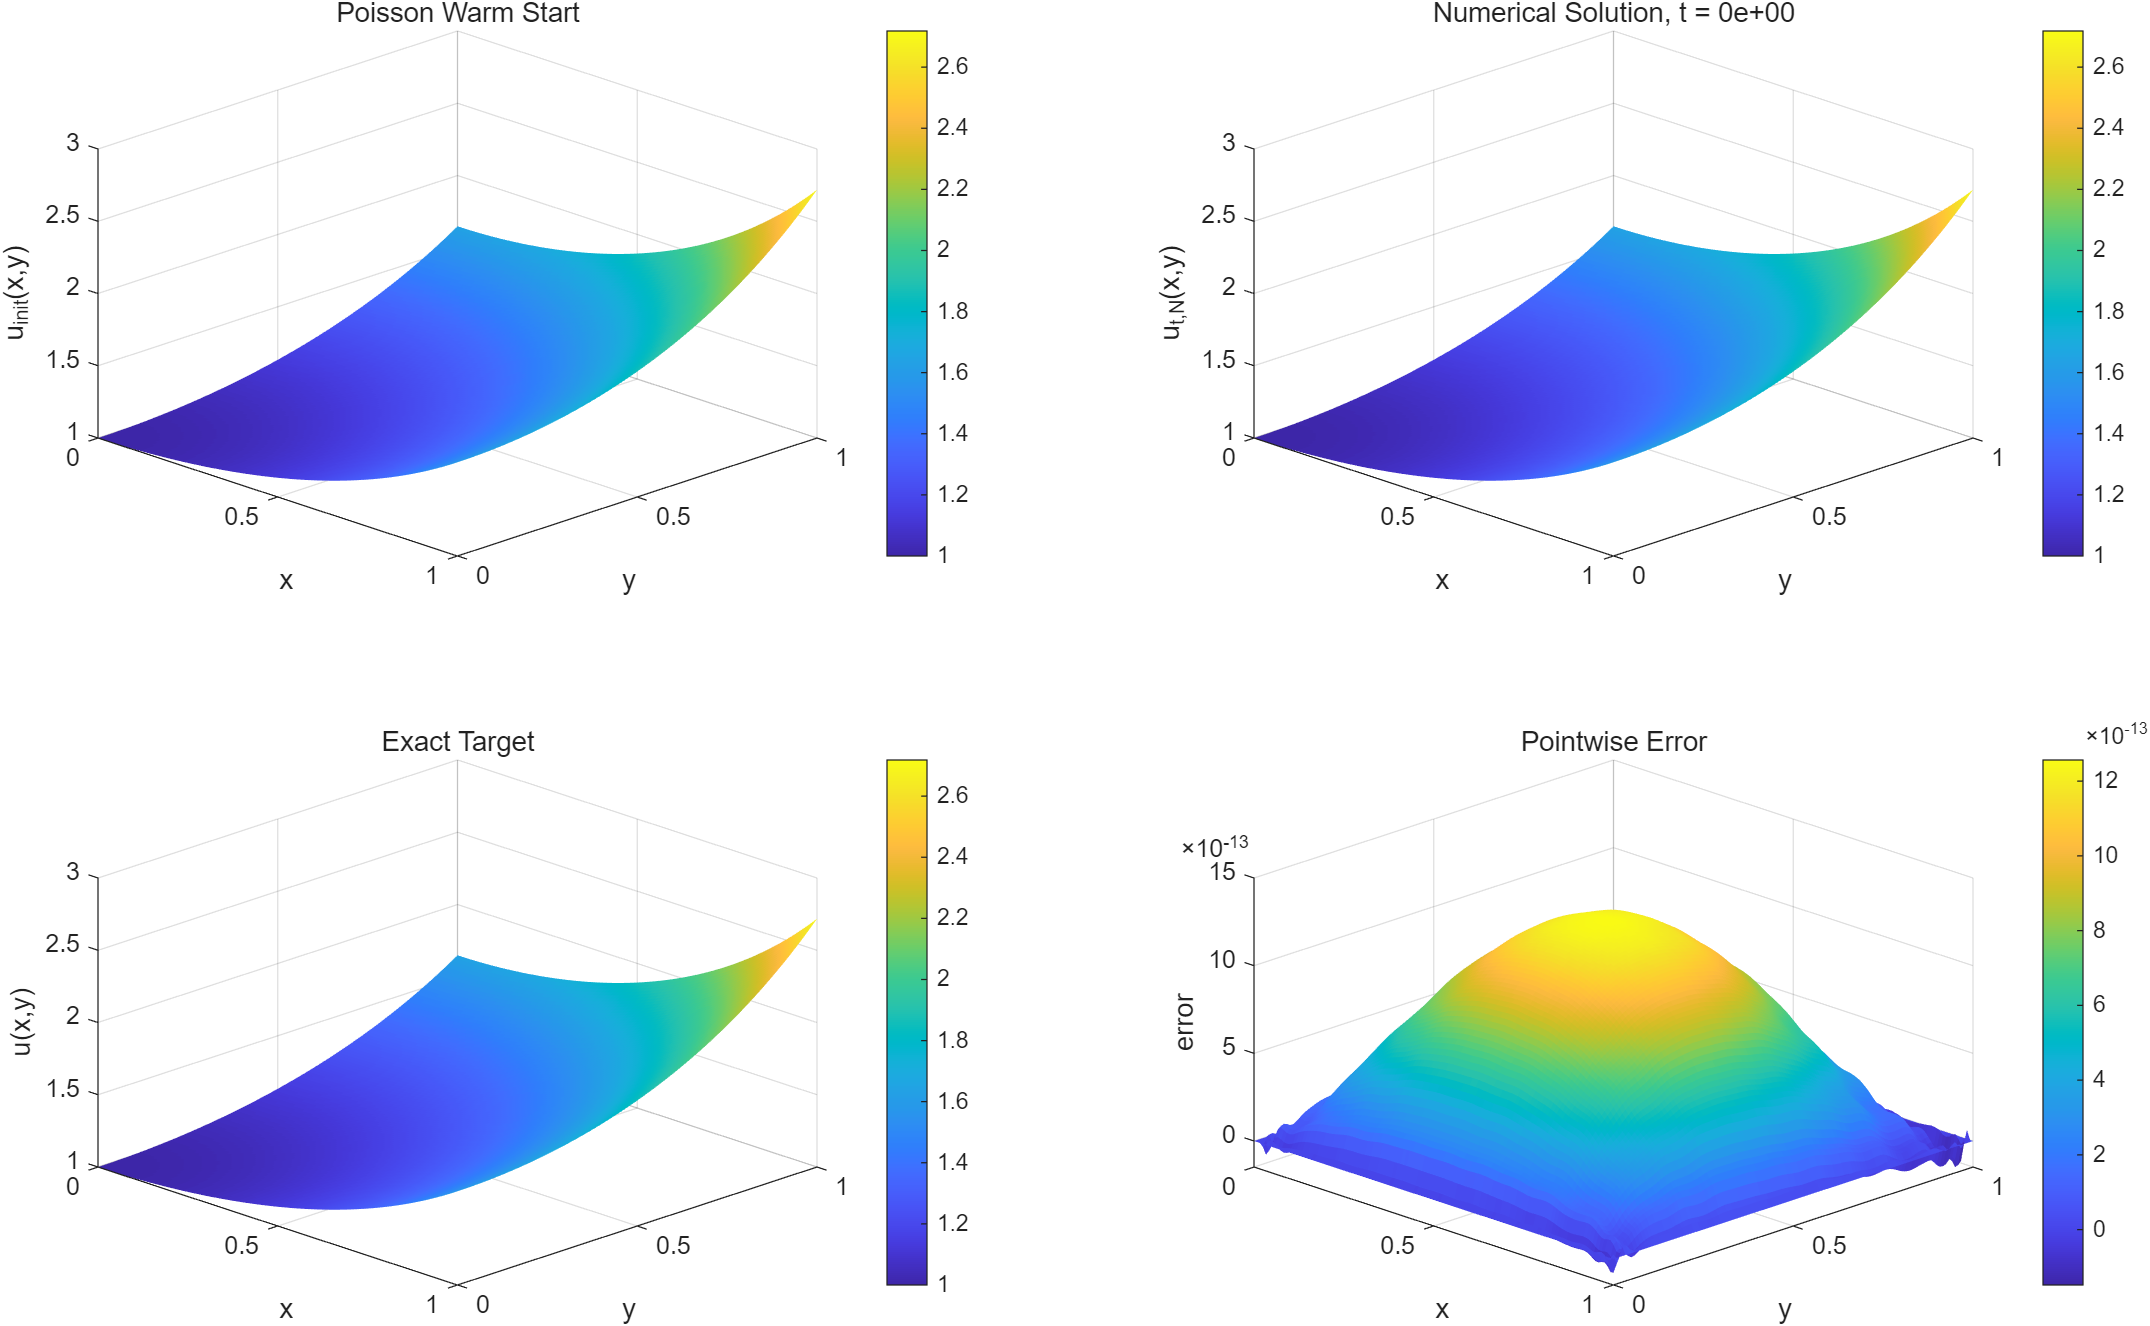
\includegraphics[width=0.88\textwidth]{output/semilinear_to_monge_ampere_homotopy_paper_example_5_1/semilinear_homotopy_surfaces.png}
\caption{\texttt{paper\_example\_5\_1} 的 Poisson warm start、最终数值解、精确解与点态误差。}
\label{fig:paper-surfaces}
\end{figure}

\begin{figure}[htbp]
\centering
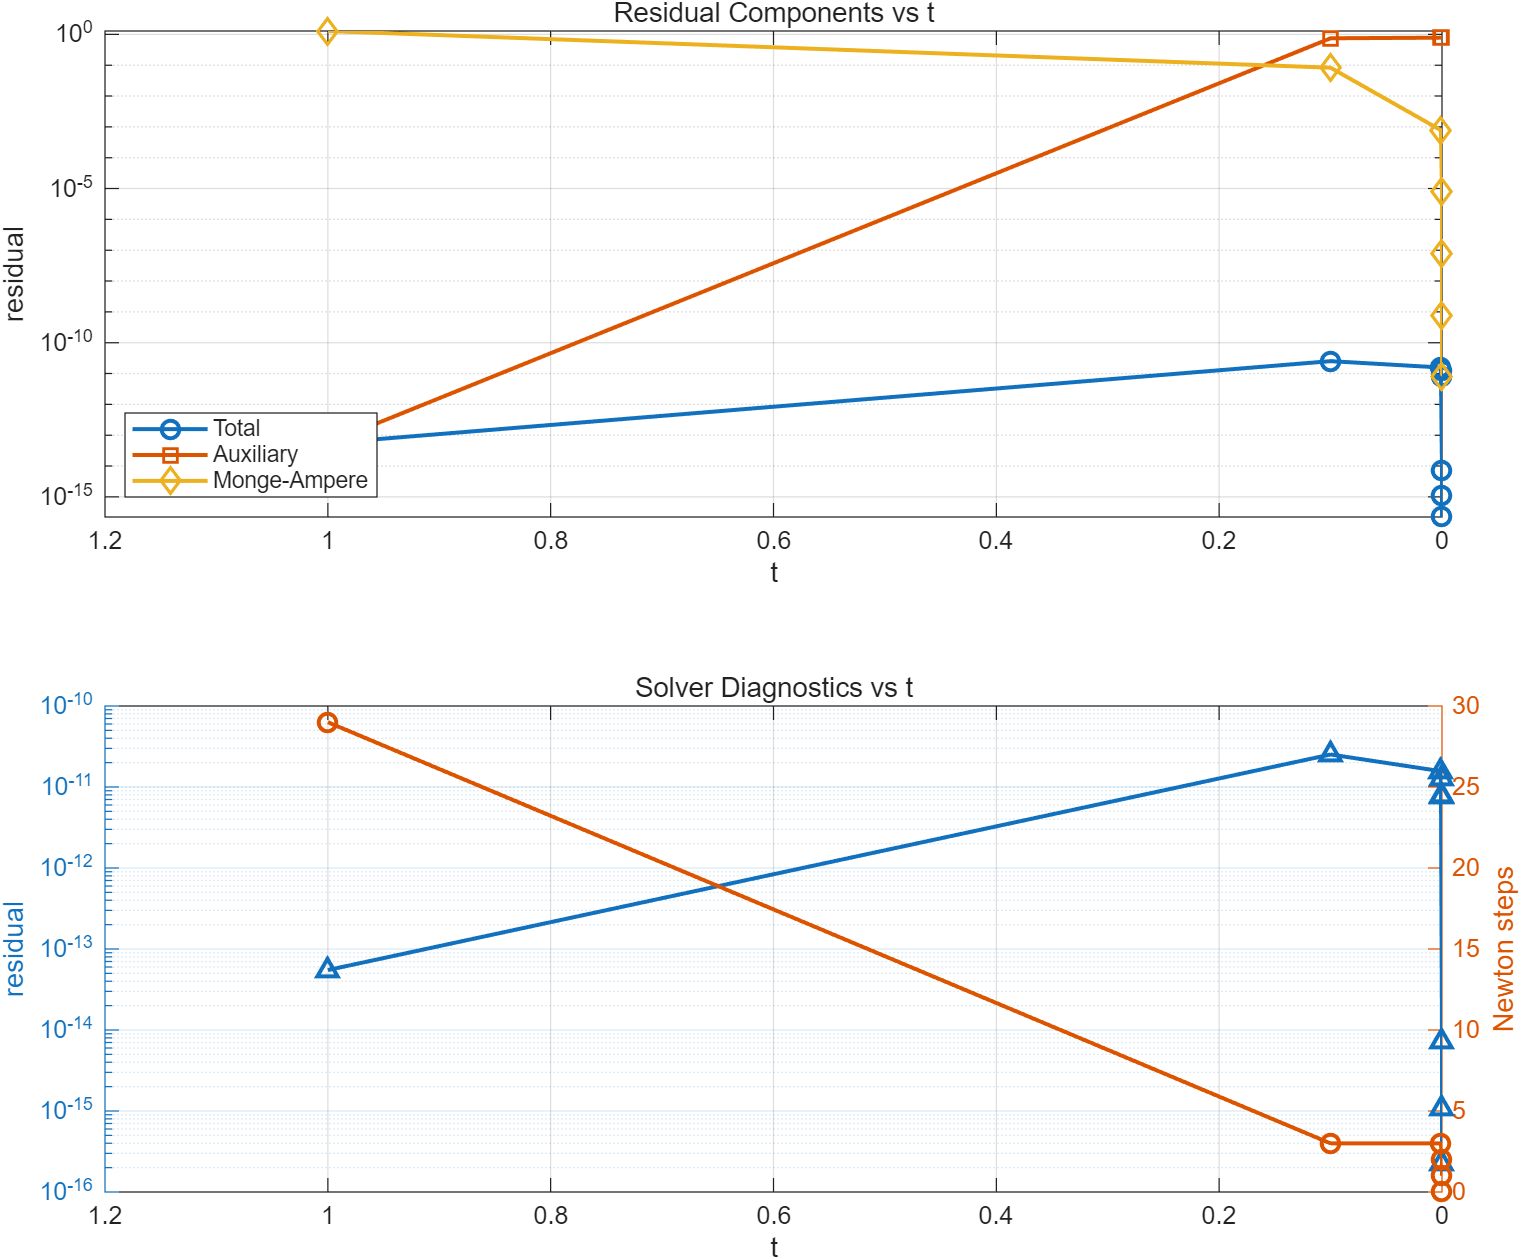
\includegraphics[width=0.82\textwidth]{output/semilinear_to_monge_ampere_homotopy_paper_example_5_1/semilinear_homotopy_solver_diagnostics.png}
\caption{\texttt{paper\_example\_5\_1} 的残差分量与求解器诊断曲线。可以看到当 $t\to 0$ 时，Monge--Amp\`ere 残差降到机器精度附近，而总残差始终保持在较低水平。}
\label{fig:paper-diagnostics}
\end{figure}

\subsection{\texorpdfstring{$quartic\_convex$}{quartic convex}: 默认参数下的失败算例}
对于 \texttt{quartic\_convex}，Poisson warm start 构造完成后，bootstrap 在第一个阶段 $s=0$ 即未能在默认最大 Newton 步数 $50$ 内收敛。此时记录到的关键量为
\[
\|R_1\|_\infty = 1.367,\qquad
\|\bm A(\bm U)\|_\infty = 1.367,\qquad
\|\bm M(\bm U)\|_\infty = 11.244.
\]
相应的误差指标为
\[
\text{Grid }L^2 = 2.991\times 10^{-1},\quad
\text{FD-}H^1 = 1.762,\quad
\text{FD-}H^2 = 15.445.
\]
此外，Hessian 最小特征值约为 $-3.807\times 10^{1}$，PSD 比例与 det-positive 比例都只有 $0.369$。这些量表明，当前 warm start 与半线性端点分支之间的距离较大，默认线搜索与凸性筛选并未能把迭代拉入一个可接受的凸性邻域。

\begin{figure}[htbp]
\centering
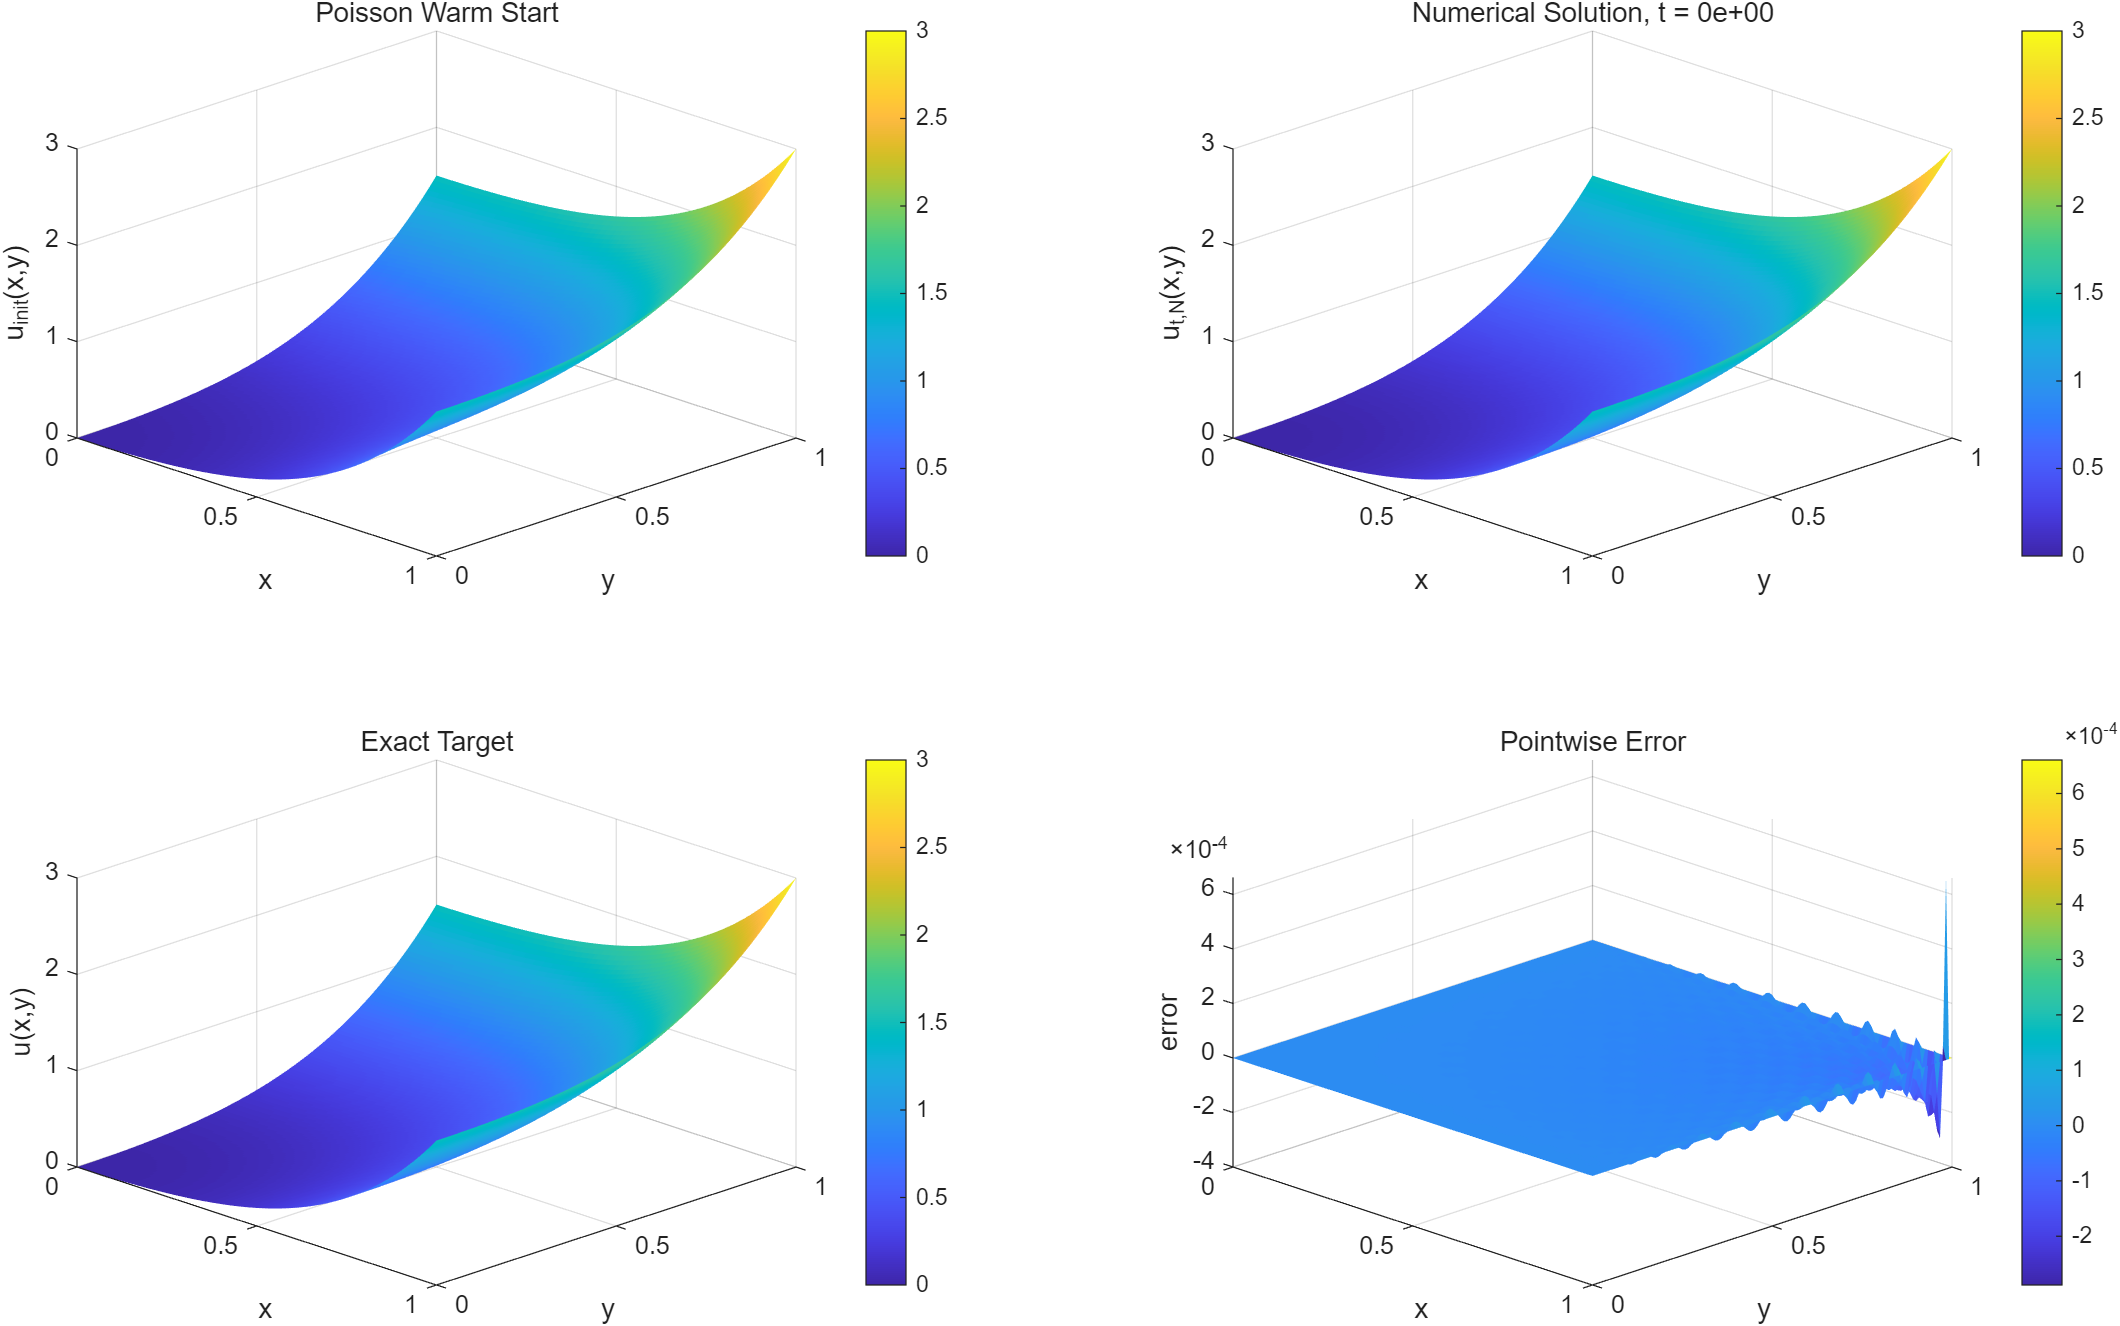
\includegraphics[width=0.88\textwidth]{output/semilinear_to_monge_ampere_homotopy_quartic_convex/semilinear_homotopy_surfaces.png}
\caption{\texttt{quartic\_convex} 在默认参数下的 Poisson warm start、停留在 $t=1$ 的数值结果、精确解与点态误差。可以看到此时仍存在明显偏差。}
\label{fig:quartic-surfaces}
\end{figure}

这一失败案例说明，新的半线性同伦路径虽然在某些光滑凸解上有效，但其半线性端点并不必然比 Monge--Amp\`ere 端点“更接近”真实分支。对于默认参数下的四次多项式凸解，初始化路径本身就可能成为算法瓶颈。

\subsection{按算例选择辅助端点的经验规则}
随着数值实验的扩展，可以看到辅助端点的选择会显著影响主同伦是否能够回到正确的凸解分支。对当前原型中的制造解算例，可将辅助端点的经验选择整理为表 \ref{tab:aux-endpoint-selection}。

\begin{table}[htbp]
\centering
\caption{不同制造解算例的辅助端点选择}
\begin{tabular}{lll}
\toprule
算例 & 当前辅助端点 & 选择依据 \\
\midrule
\texttt{paper\_example\_5\_1} & $\Delta u + u^3 = f$ & 半线性端点与目标凸分支匹配较好 \\
\texttt{quartic\_convex} & $\Delta u + u^3 = f$ & 配合 bootstrap 后仍可接回目标分支 \\
\texttt{scaled\_quartic\_convex} & $\Delta u + u^3 = f$ & 数据幅值较温和，半线性路径稳定 \\
\texttt{trig\_convex} & $\Delta u + u^3 = f$ & 可作为振荡型凸解的验证算例 \\
\texttt{mild\_sextic\_convex} & $\Delta u + u^3 = f$ & 六次分离变量结构下路径稳定且误差较低 \\
\texttt{mixed\_polynomial\_convex} & $\Delta u + u^3 = f$ & 在新 bootstrap 规则下可稳定收敛 \\
\texttt{gaussian\_bump\_convex} & $\Delta u + u^3 = f$ & 局部高斯凸包算例在新规则下可稳定收敛 \\
\texttt{mild\_exp\_separable} & $\Delta u = 2\sqrt{f}$ & $f$ 很小，$u^3$ 相对过强，需改用 Poisson 型端点 \\
\bottomrule
\end{tabular}
\label{tab:aux-endpoint-selection}
\end{table}

从表 \ref{tab:aux-endpoint-selection} 可以看出，当前默认的半线性端点
\[
\Delta u + u^3 = f
\]
适用于大多数中等幅值、目标凸分支较容易恢复的算例；但当 Monge--Amp\`ere 右端 $f$ 很小而 $u^3$ 项相对偏强时，半线性端点可能把 $t=1$ 层解拉向错误分支。对于这类算例，更自然的做法是改用与 Hessian 行列式尺度更贴近的 Poisson 型端点
\[
\Delta u = 2\sqrt{f},
\]
从而在 continuation 之前就把初始端点放在更接近目标凸解的邻域内。数值上，\texttt{mild\_exp\_separable} 正是这一经验规则的代表性例子。

\section{局限性与结论}
从上述两组算例看，这个新 demo 已经具备较清晰的数学结构：连续模型明确，残差与 Jacobian 都可以解析组装，数值诊断量也较丰富。然而，它当前仍然只是研究型原型，主要局限体现在以下几个方面：
\begin{itemize}[leftmargin=2em]
\item 半线性端点 $\Delta u+u^3=f$ 是否总能提供一条良好的同伦路径，目前缺乏理论保证；
\item bootstrap 阶段对 warm start 和线搜索较敏感，四次多项式凸解在默认配置下即告失败；
\item 现有凸性控制主要是经验性的接受准则，而非严格的分支保持理论；
\item 当前方法仍建立在矩形区域上的张量积 Legendre--Galerkin 框架内，对更复杂几何尚未处理。
\end{itemize}

综上，本文整理了一种从半线性端点到 Monge--Amp\`ere 方程的同伦 Legendre--Galerkin 原型方法。其主要特征在于：首先通过 Poisson 方程构造 warm start；其次借助 bootstrap 方程族逐步建立半线性端点初值；最后再沿参数 $t$ 从半线性模型连续过渡到 Monge--Amp\`ere 模型。离散层面上，方法继续沿用稳定的 B-matrix 变换链，并对半线性项与 Hessian 行列式项分别构造解析 Jacobian。数值实验表明，该路径对指数型光滑凸解非常有效，但对四次多项式凸解在当前默认参数下仍存在明显困难。因而，这一新同伦方法更适合被看作后续研究更稳健初始化与分支控制策略的出发点，而不是已经成熟的通用求解器。

\end{document}
